\documentclass{article}
\usepackage[utf8]{inputenc}

\title{%
  Sistema de Avaliação de Discente\\
  \large utilizando lógica\\
    Fuzzy}

\author{Daniel Ferreira, Ivan Carlos, Rodrigo de Paula} 
\date{October 2021}

\usepackage{natbib}

\usepackage{blindtext} % links
\usepackage{hyperref}  % links

\usepackage{graphicx}
\usepackage{geometry}
\usepackage[utf8]{inputenc}
\usepackage[T1]{fontenc}
\usepackage[brazil]{babel}

%\geometry{left=2.5cm,right=2.5cm,top=2.5cm,bottom=2.5cm}

\begin{document}

\maketitle

\section{Descrição do trabalho}

O trabalho consiste em projetar, implementar e mostrar
funcionando um sistema de avaliação que utilize lógica difusa
(fuzzy), para gerar a média final dos alunos de uma determida
disciplina fictícia. É permitido escolher as variáveis de
entrada suas funções de pertinência, variáveis de saída e
suas respectivas funções de pertinência e regras do sistema.

\section{Introdução}

``Os sistemas especialistas são programas de computador que
emulam o processo de raciocínio de um especialista humano ou
atuam de maneira especializada em um domínio para o qual não
existe nenhum especialista humano. Eles normalmente raciocinam
com informações incertas e imprecisas. Existem muitas fontes
de imprecisão e incerteza. O conhecimento que eles incorporam
muitas vezes não é exato, da mesma forma que o conhecimento de
um humano é imperfeito. Os fatos ou informações fornecidas
pelo usuário também são incertos.

Sistemas especialistas são programas de computador que emulam
o processo de raciocínio de um especialista humano ou atuam
em um sistema especialista expert. Normalmente, é composto de
pelo menos três partes: um mecanismo de inferência, uma base
de conhecimento e uma memória global ou de trabalho. A base de
conhecimento contém o conhecimento de domínio especializado
para uso na solução de problemas. A memória de trabalho é
usada como bloco de rascunho e para armazenar informações
obtidas do usuário do sistema. O mecanismo de inferência usa o
conhecimento do domínio junto com as informações adquiridas
sobre um problema para fornecer uma solução especializada.

Os sistemas especialistas modelaram a incerteza e a imprecisão
de várias maneiras. A maioria dos métodos de lidar com a
incerteza e imprecisão em sistemas especialistas tem sido ad
hoc, no sentido de que não existe uma teoria subjacente para
apoiá-los. Eles foram validados apenas por meio de testes
empíricos.

Eles geralmente usam alguma forma de regras de alto nível. A
busca cega do espaço da solução é evitada e alto desempenho,
se aproximando ou ultrapassando o de um especialista, é
obtido. O raciocínio pode ser feito por manipulação de
símbolo. Eles mostram alguma inteligência. Os sistemas
especialistas incorporam princípios de domínio fundamentais
e métodos de raciocínio fracos. Eles têm dificuldade ou
complexidade associada a eles. Eles podem reformular um
problema e alguma razão sobre si mesmos. Eles podem ser
descritos como programas de computador que usam conhecimento de
domínio e técnicas de raciocínio para resolver problemas que
normalmente requerem um especialista humano para sua solução.
Os sistemas especialistas podem realizar uma tarefa que os
humanos normalmente não realizam, como a orientação de
mísseis ou o planejamento de um robô. Um sistema especialista
pode ser capaz de atuar habilmente em uma área na qual não há
especialistas humanos.''\citep{kandel1992fuzzy}

\section{Projetando um sistema de avaliação de discentes}

O sistema de avaliação utilizado nas disciplinas é geralmente 
baseado por avaliações escritas que são aplicadas ao término 
de cada unidade ou conteúdo. O planejamento da quantidade 
de provas depende de cada instituição e professor. De uma 
forma geral, são duas provas por semestre ou no máximo três 
provas, onde cada uma avalia um determinado conteúdo. Após a 
realização de cada exame o aluno obtém uma nota. No final de 
um determinado período é feita uma média aritmética com
todas as notas do aluno. A média final para a aprovação é
determinada pela instituição.

O cálculo matemático utilizado não deixa claro o conhecimento
que o aluno realmente adquiriu. Ele pode ter tido uma nota
excelente na prova referente ao conteúdo de X, por
exemplo, e uma nota ruim na prova de conteúdo Y, mas 
calculando sua média obteve-se uma nota suficiente para aprovação.

Como conseqüência, o aluno será aprovado por ter bastante
conhecimento em X, mas terá uma dificuldade em Y.

No exemplo citado, após o resultado da avaliação do aluno
não é feita uma retomada dos conteúdos em que os alunos
apresentaram maiores problemas. A respeito
da dificuldade em Y. Já que o aluno foi aprovado, não 
se preocupa se o conhecimento adquirido é satisfatório 
para prosseguir nas disciplinas subsequentes.

\section{Métodos de inferência (Máquinas de inferência)}

Os 2 tipos mais importantes de método de inferência fuzzy
são \emph{Mamdani} e \emph{Sugeno}. O método de inferência 
difuso do tipo Mamdani é o método mais comumente usado. 
Este método foi introduzido por Mamdani e Assilian (1975). 
Outro método de inferência bem conhecido é o chamado método do processo de inferência fuzzy Sugeno ou Takagi-Sugeno-Kang. 
Este método foi introduzido por Sugeno (1985). Este método 
também é chamado de método TS. A principal diferença entre 
os dois métodos reside no consequente das regras Fuzzy.


\subsubsection{Método de Inferência Difusa Mamdani\citep{
ProfVolmirWilhelm}}

Etapas:

\begin{enumerate}
    \item  Determinar um conjunto de regras fuzzy
    \item  Fuzzificar das entradas usando as funções de pertinência de entrada;
    \item  Combinar as entradas fuzificadas de acordo com as regras fuzzy para
estabelecer a ``força da regra'' (operações difusas);
    \item  Encontrado o resultado da regra, combinar a ``força da regra'' com a função
de pertinência de saída (implicação);
    \item  Combinar as consequências para obter uma saída (agregação);
    \item  Defuzzificar a saída (apenas se uma saída crisp é necessária).
\end{enumerate}







\begin{figure}[h!]
\centering
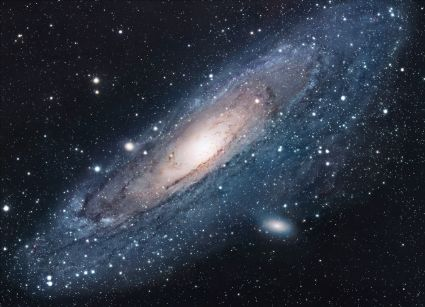
\includegraphics[scale=1.7]{universe.jpg}
\caption{The Universe}
\label{fig:univerise}
\end{figure}

\section{Conclusão}
Sabemos que a função da avaliação é auxiliar o processo de
ensino/aprendizagem dos alunos, porém a maneira que está sendo
aplicada não está surtindo os resultados esperados. Para obter
o conceito final do desempenho do aluno, após a realização
de todas as provas de um determinado período, é calculada a
média aritmética com todas as notas obtidas.

A média aritmética usada para o cálculo da nota final
do aluno não analisa todas as notas em conjunto. Um aluno
conseguiu boas notas na primeira e na segunda prova, porém
na terceira prova ele obteve uma nota inferior. Ao calcular
a média esta diminui consideravelmente por causa da nota
baixa da terceira prova. No caso de uma nota mais baixa ao
fazer o cálculo da média o aluno pode ser prejudicado mesmo
tendo notas boas em outras provas. Uma média insatisfatória
transparece que o aluno não aprendeu. Ele pode ter aprendido
muito bem o conteúdo da primeira e segunda prova, porém ele
ficou com uma deficiência no conteúdo da terceira prova. A
média aritmética não mostra essa realidade.


As provas aplicadas e o cálculo matemático utilizado estão
sendo insuficientes para avaliar o aprendizado dos alunos,
portanto um modelo fuzzy foi desenvolvido neste trabalho
utilizando o software Matlab visando a avaliação para cursos
presenciais.


A lógica fuzzy é uma abordagem intuitiva e tolerante com dados
imprecisos. Pode ser construída através de experiência de
especialistas e sobre as estruturas da descrição qualitativa
utilizada na linguagem cotidiana.

Em nosso modelo utilizamos valores aleatórios como entrada
para o sistema fuzzy, tentando contemplar a maior quantidade
possível de situações para avaliar o desempenho dos alunos.
Estes valores utilizados são: nota de avaliação escrita,
atividade em classe e atividade extra classe. O principal
objetivo era usar todos os tipos de avaliações para estimar
um novo índice para o conceito final dos alunos e comparar os
resultados obtidos com o modelo clássico (cálculo matemático
– média aritmética). O sistema fuzzy tem algumas vantagens
quando comparado com o modelo clássico. Possui muitos recursos
para aperfeiçoar a modelagem e adquirir melhores resultados,
por exemplo o formato das funções de pertinência, o modelo de
inferência que pode ser o Mamdani ou o Sugeno além de permitir
trabalhar com variáveis quantitativas e qualitativas. Para
a modelagem desse sistema foi construída uma base de regras
através de variáveis linguísticas que pode ser modificada
até adquirir os resultados esperados. O modelo desenvolvido
possui 20 regras para estimar o índice e sua implementação e
interpretação são fáceis para o usuário.


O mais importante é que este sistema considera a contribuição
de todas as etapas de avaliação do aluno para gerar o índice
para o conceito final. Esta importante contribuição não
ocorreu com os modelos clássicos, porque eles prejudicam o
conceito final do aluno que não foi muito bem em umas das
etapas de avaliação.


Dentre os testes que podem ser feitos no modelo fuzzy como
proposta de trabalhos futuros são: 

\begin{itemize}
    \item Dar pesos diferentes para uma determinada regra;
    \item Ao invés de utilizar o método de implicação
Mamdani pode ser usado o modelo de Takagi-Sugeno-Kang;
    \item Além da trapezoidal pode utilizar outras formas de
    funções de pertinência como a triangular, gaussiana,
    sinoidal;
    \item Diminuir as regras para obter melhores resultados.
\end{itemize}

Assim, a metodologia proposta sugere um novo índice de
cálculo que foi capaz de melhorar os resultados do sistema
de classificação clássico na maioria das situações
simuladas e tem uma grande flexibilidade. Estes elementos
ampliam significativamente a sensibilidade do modelo para
a classificação do conceito final do estudante, e faz da
metodologia uma proposta muito adaptável a qualquer nova norma.
	


\bibliographystyle{plain}
\bibliography{references}

\end{document}
